\documentclass[12pt]{article}
\usepackage{class/sbc-template}
\usepackage{graphicx,url}
\usepackage[utf8]{inputenc}
\usepackage[brazil]{babel}
\usepackage{color}
\usepackage{listings}

%%%%%%%%%%%%%%%%%%%%%%%%%%%%%%%%%%%%%%%%%%%%%%%%%%%%
% C O N F I G U R A Ç Õ E S  D O S   C Ó D I G O S %
%%%%%%%%%%%%%%%%%%%%%%%%%%%%%%%%%%%%%%%%%%%%%%%%%%%%

\lstset{
	numbers=left,
	stepnumber=1,
	firstnumber=1,
	numberstyle=\tiny,
	extendedchars=true,
	breaklines=true,
	frame=single,
	showstringspaces=false,
	xleftmargin=2.5em,
	framexleftmargin=2em,
	basicstyle=\small,
}

\renewcommand{\lstlistingname}{Código}
\renewcommand{\lstlistlistingname}{Lista de Códigos}

\sloppy

\title{Aprendizagem de Máquina (2020/Período Especial) - Impactos da Base de Aprendizagem}

\author{Diogo C. T. Batista\inst{1}}

\address{Universidade Federal do Paraná (UFPR)\\
	Curitiba -- Paraná -- Brasil
	\email{diogo@diogocezar.com}
	}

\begin{document}

\maketitle

\section{Impactos da Base de Aprendizagem}

Esta atividade laboratorial tem como objetivo a investigação exploratória dos impáctos da base de aprendizagem na performance de diferentes classificadores. Os classificadores a serem analisados neste laboratório são:

\begin{itemize}
  \item KNN
  \item Naïve Bayes
  \item Linear Discriminant Analysis
  \item Logistic Regression
  \item Perceptron
\end{itemize}

Os dados estão dispostos em arquivo no formato \textit{svmlight}. Este formato dispõe as informações de categorias e suas respectivas características. O código \ref{code:svmlight} mostra um pequeno trecho desta representação.

\begin{lstlisting}[caption={Exemplo do Formato de Entrada},captionpos=b,frame=single,label={code:svmlight}]
0 1:0.000000 2:0.000000 3:0.001412 4:0.000000 5:0.014124 6:0.000000 ...
\end{lstlisting}

Neste exemplo, podemos notar que o $0$ inicial mostra a qual categoria este dado pertence, na sequência, demonstra-se para cada característica o seu valor. A característica $1$ possui o valor $0.000000$.

Os dados utilizados neste experimento estão dividos em 2 partições. A primeira partição possui $20.000$ registros, que foi definida para uma base de treinamento. Já a segunda, possui $58.646$ informações, utilizadas para o teste.

\subsection{Estratégia para Execução do Experimento}

Para automatização da suite de experimentos, foi criado um sistema \textit{orquestrador} no qual é possível definir quais vão ser os experimentos a serem executados. O Código \ref{code:orquestrador} mostra os valores definidos em um arquivo no formato \textit{JSON}.

\begin{lstlisting}[caption={JSON do Orquestrador},captionpos=b,frame=single,label={code:orquestrador}]
[
  {
    "classifier": "knn",
    "chunk_start": 1000,
    "chunk_stop": 20000,
    "chunk_step": 1000
  },
  {
    "classifier": "naive\_bayes",
    "chunk_start": 1000,
    "chunk_stop": 20000,
    "chunk_step": 1000
  },
  ...
]
\end{lstlisting}

Neste JSON, \textit{classifier} é o nome do classificador a ser utilizado. Estes, podem variar entre: knn, naive\_bayes, lda, logistic\_regression, e perceptron. Os outros atributos servem parar criar chunks que dividem os testes em função da disponibilidade da base de treinamento. Por exemplo, no primeiro bloco, \textit{chunk\_start} indica o tamanho do bloco inicial, \textit{chunk\_stop} indica a condição de parada, e por fim o \textit{chunk\_step} indica o incremento.

Para os testes, em todos os classificados variou-se a base de treinamento de $1000$ até $20000$, com o intervalo de $1000$.

O script implementado ainda realiza a automação da coleta dos resultados, salvando em arquivo no formato \textit{csv} todos os dados extraídos dos experimentos.

Os dados salvos são: \textit{Classifier}, \textit{Chunk}, \textit{F1Score}, \textit{Accuracy} e \textit{Execution Time (s)}.

\subsection{Parametrização dos Classificadores}

Para este trabalho, foram implementados os parâmetros padrões para todos os classificadores anteriormente descritos. Assim sendo, nenhum ajuste específico foi realizado qualquer um dos classificadores testados.

\subsection{Experimentos}

Foram realizados $100$ experimentos. $20$ variação de $1000~20000$ para cada um dos 5 classificadores. Os $20$ melhores resultados estão demonstrados por ordem de \textit{F1Score} seguidos de \textit{Acurácia} e o \textit{Tempo de Execução} na tabela \ref{tab:resultados_melhores}

\begin{table}[!htb]
  \centering
\begin{tabular}{|c|c|c|c|c|}
\hline
\textbf{Classifier} & \textbf{Chunk} & \textbf{F1Score} & \textbf{Accuracy} & \textbf{Execution Time (s)} \\ \hline
knn                 & 20.000         & 0,939            & 0,939             & 292,836                     \\ \hline
perceptron          & 11.000         & 0,938            & 0,938             & 5,501                       \\ \hline
knn                 & 19.000         & 0,938            & 0,938             & 279,718                     \\ \hline
knn                 & 18.000         & 0,938            & 0,937             & 268,223                     \\ \hline
knn                 & 16.000         & 0,937            & 0,937             & 251,132                     \\ \hline
knn                 & 17.000         & 0,937            & 0,937             & 257,359                     \\ \hline
knn                 & 12.000         & 0,936            & 0,936             & 225,239                     \\ \hline
knn                 & 13.000         & 0,936            & 0,936             & 237,264                     \\ \hline
knn                 & 14.000         & 0,936            & 0,936             & 253,580                     \\ \hline
knn                 & 15.000         & 0,936            & 0,935             & 270,468                     \\ \hline
perceptron          & 17.000         & 0,935            & 0,935             & 5,710                       \\ \hline
knn                 & 10.000         & 0,935            & 0,935             & 198,619                     \\ \hline
knn                 & 11.000         & 0,935            & 0,934             & 210,219                     \\ \hline
perceptron          & 18.000         & 0,934            & 0,934             & 5,717                       \\ \hline
knn                 & 9.000          & 0,933            & 0,933             & 178,040                     \\ \hline
knn                 & 8.000          & 0,930            & 0,929             & 157,567                     \\ \hline
lda                 & 10.000         & 0,928            & 0,928             & 5,030                       \\ \hline
perceptron          & 13.000         & 0,928            & 0,928             & 5,337                       \\ \hline
lda                 & 20.000         & 0,928            & 0,928             & 5,403                       \\ \hline
perceptron          & 20.000         & 0,926            & 0,927             & 5,677                       \\ \hline
\end{tabular}
  \caption{Melhores Resultados}
  \label{tab:resultados_melhores}
\end{table}

\subsection{Análises dos Resultados}

A análise dos resultados leva em considerações os quesitos:

\begin{enumerate}
  \item Comparação do Desempenho dos Classificadores;
  \item Classificador que tem o melhor desempenho com poucos dados;
  \item Classificador que tem melhor desempenho com todos os dados;
  \item Classiticador mais rápido;
  \item Análise das Matrizes de Confusão;
\end{enumerate}

\subsubsection{Comparação do Desempenho dos Classificadores}

A figura 

\begin{figure}[!htb]
  \centering
  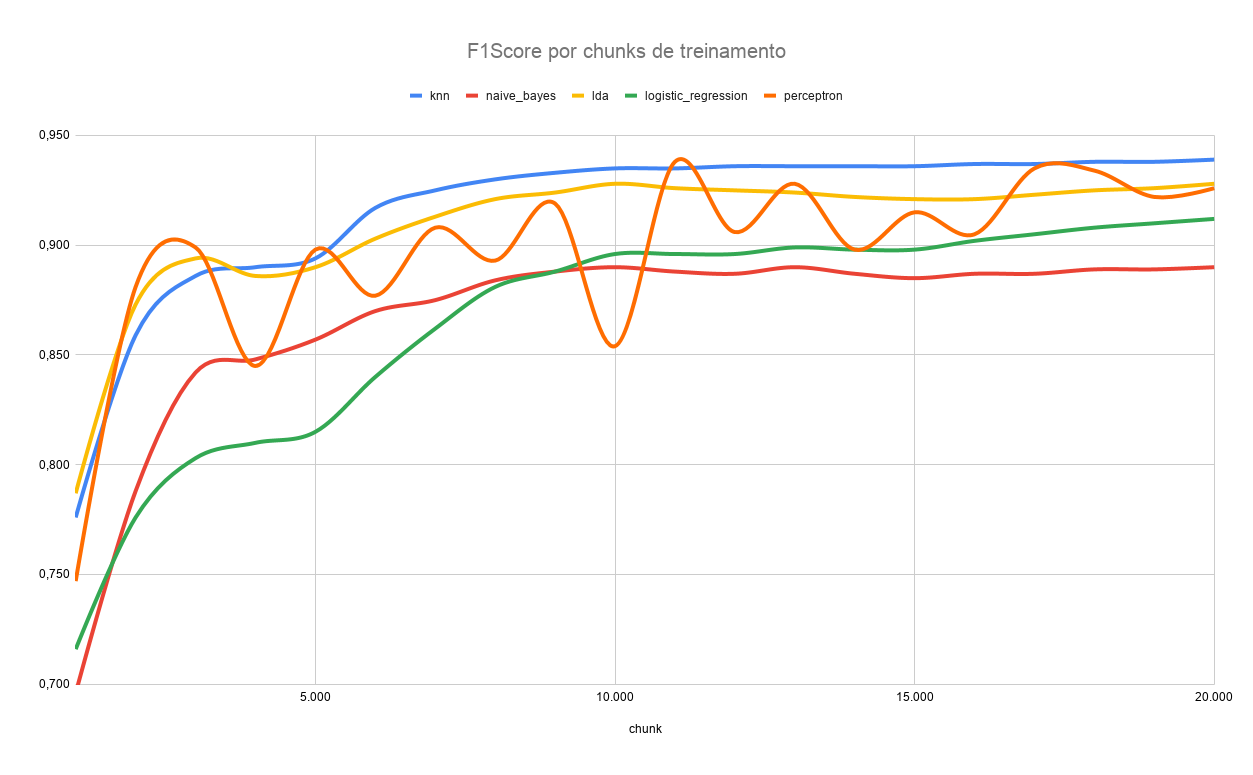
\includegraphics[width=30em]{images/image_comparacao_classificadores.png}
  \caption{Comparação de Desempenho dos Classificadores}
  \label{fig:comparacao_classificadores}
\end{figure}

\section{Experimentos}

Assim como na adaptação do primeiro algoritmo, um sistema de entrada JSON possibilitou a variação de combinações para análise de diferentes resultados.

\begin{itemize}
  \item O arquivo de representação fonte; as variações testadas foram: [features\_20\_10, features\_36\_46, features\_40\_20, features\_60\_30, features\_99\_81]
  \item Ativar ou desativar a normalização; as variações testadas foram: [0,1]
  \item Alterar o tipo de distância; as variações testadas foram: [eucledian, manhattan]
  \item Alterar o K; as variações testadas foram: [1,3,4,5,6,7,8,9,10,11,12,13]. Foram considerados os $K$ pares, apenas para efeito de comparações, sabendo-se se sua ineficiência por natureza.
\end{itemize}

\newpage

O Código \ref{code:json_experimentos} mostra as opções de entrada para o algorítmo, podendo variar:

\begin{lstlisting}[caption={JSON para experimentos},captionpos=b,frame=single,label={code:json_experimentos}]
[
  {
    "data": "features_20_10",
    "normalized": 0,
    "distance": "euclidean",
    "k": 1
  },
  ...
]
\end{lstlisting}

\section{Resultados}

Foram realizadas \textit{240} execuções para as variações listadas anteriormente. Os \textit{20} melhores resultados (ordenados por Acurácia e F1Score) estão detalhados na Tabela \ref{tab:resultados_melhores}. Já os 20 piores resultados (ordenados por Acurácia e F1Score) estão detalhados na Tabela \ref{tab:resultados_piores}.

Pode-se observar que os melhores resultados foram obtidos a partir das representações que consideraram as \textit{maiores} alturas e larguras das imagens (99x81). Isso acontece pois, no momento em que se realiza a compressão das imagens, características são perdidas. O melhor resultado teve a \textit{Acurácia} de $0,928$ e o \textit{F1Score} de $0,929$ demorando $2.743$ segundos para execução completa.

Já para nos piores resultados, nota-se que foram obtidos na variação de K: $K=13$, $K=12$, $K=10$. Quanto ao $K$ para os melhores resultados, percebe-se que foram obtidos com $K=1$, seguido de $K=3$ e $K=5$. Isso mostra que a distribuição possui uma particularidade interessante, na qual ao se comparar apenas os vizinhos mais próximos se consegue um melhor resultado. Como já esperado, para os resultados nos quais $K$ tinha um valor par, seus resultados foram menos eficientes.

Em outra análise, a estratégia de obter as médias das alturas e larguras também apresentaram resultados significativos (imagens de dimensão $36x46$), mas ficaram abaixo dos resultados da estratégia empírica que utiliza imagens $60x30$. O destaque é para o tempo de execução em \textit{features\_60\_30}, que conseguiu-se uma Acurácia de $0,925$ e o F1Score de $0,926$ demorando apenas $203$ segundos para execução completa.

As normalizações não parecem fazer muita diferença nos resultados, pois estes já se encontram bem distribuídos.

Em geral a alteração da estratégia de medição das distâncias (\textit{euclidean} e \textit{manhattan}) não influenciaram em uma melhoria da \textit{Acurácia} ou do \textit{F1Score}. O que se pode notar, foi que nos testes executados a estratégia \textit{manhattan} impacta negativamente no tempo de execução.



\begin{table}[!htb]
  \centering
  \begin{tabular}{|c|c|c|c|c|c|c|}
  \hline
  \textbf{Experiment} & \textbf{Normalized} & \textbf{Distance} & \textbf{K} & \textbf{Accuracy} & \textbf{F1Score} & \textbf{Execution Time (s)} \\ \hline
  features\_20\_10    & 1                   & manhattan         & 13         & 0,871             & 0,873            & 40                          \\ \hline
  features\_20\_10    & 1                   & euclidean         & 13         & 0,871             & 0,873            & 30                          \\ \hline
  features\_20\_10    & 0                   & manhattan         & 13         & 0,871             & 0,873            & 20                          \\ \hline
  features\_20\_10    & 0                   & euclidean         & 13         & 0,871             & 0,873            & 10                          \\ \hline
  features\_20\_10    & 1                   & manhattan         & 12         & 0,874             & 0,876            & 39                          \\ \hline
  features\_20\_10    & 1                   & euclidean         & 12         & 0,874             & 0,876            & 29                          \\ \hline
  features\_20\_10    & 0                   & manhattan         & 12         & 0,874             & 0,876            & 19                          \\ \hline
  features\_20\_10    & 0                   & euclidean         & 12         & 0,874             & 0,876            & 9                           \\ \hline
  features\_99\_81    & 1                   & manhattan         & 12         & 0,876             & 0,879            & 4.294                       \\ \hline
  features\_99\_81    & 1                   & euclidean         & 12         & 0,876             & 0,879            & 3.894                       \\ \hline
  features\_99\_81    & 0                   & manhattan         & 12         & 0,876             & 0,879            & 3.485                       \\ \hline
  features\_99\_81    & 0                   & euclidean         & 12         & 0,876             & 0,879            & 3.090                       \\ \hline
  features\_20\_10    & 1                   & manhattan         & 10         & 0,879             & 0,881            & 37                          \\ \hline
  features\_20\_10    & 1                   & euclidean         & 10         & 0,879             & 0,881            & 27                          \\ \hline
  features\_20\_10    & 0                   & manhattan         & 10         & 0,879             & 0,881            & 17                          \\ \hline
  features\_20\_10    & 0                   & euclidean         & 10         & 0,879             & 0,881            & 7                           \\ \hline
  features\_99\_81    & 1                   & manhattan         & 13         & 0,880             & 0,883            & 4.328                       \\ \hline
  features\_99\_81    & 1                   & euclidean         & 13         & 0,880             & 0,883            & 3.928                       \\ \hline
  features\_99\_81    & 0                   & manhattan         & 13         & 0,880             & 0,883            & 3.517                       \\ \hline
  features\_99\_81    & 0                   & euclidean         & 13         & 0,880             & 0,883            & 3.126                       \\ \hline
  \end{tabular}
  \caption{Piores Resultados}
  \label{tab:resultados_piores}
\end{table}

\section{Comparação das Matrizes de Confusão}

Para cada execução, criou-se um arquivo de resultados que também armazena as matrizes de confusão.

A Tabela \ref{tab:matriz_confusao_melhor} demonstra a matriz de confusão para o melhor resultado, enquanto que a Tabela \ref{tab:matriz_confusao_pior} demonstra a matriz de confusão para o pior resultado.

É possível notar que apesar dos erros persistirem na classificação, como por exemplo em: [0,2],[1,2],[1,3],[1,4],[1,6],[1,7],[1,8],[1,9], eles diminuram consideravelmente. Como por exemplo, no pior caso, a classificação [1,4] foi classificada erroniamente 12 vezes, enquanto que no melhor caso, o erro ocorreu em apenas 8 vezes. Isso acontece, pois, aumentar o número de \textit{pixels} analisados nas imagens, geram representações mais precisas, porém, como o método é o mesmo, pôde-se observar que os equívocos continuaram existindo nos mesmos lugares, mesmo que em menor número.

\begin{table}[!htb]
  \centering
  \begin{tabular}{|c|c|c|c|c|c|c|c|c|c|}
  \hline
  95 & 0  & 0   & 0  & 0  & 1  & 1   & 0  & 0  & 0   \\ \hline
  0  & 93 & 0   & 0  & 0  & 1  & 0   & 0  & 0  & 1   \\ \hline
  0  & 1  & 103 & 1  & 0  & 0  & 0   & 4  & 1  & 1   \\ \hline
  0  & 1  & 0   & 98 & 0  & 1  & 0   & 0  & 3  & 0   \\ \hline
  0  & 8  & 0   & 0  & 83 & 1  & 1   & 0  & 0  & 2   \\ \hline
  2  & 0  & 0   & 5  & 0  & 89 & 1   & 0  & 0  & 0   \\ \hline
  1  & 5  & 0   & 0  & 0  & 0  & 100 & 0  & 0  & 0   \\ \hline
  0  & 3  & 1   & 0  & 1  & 0  & 0   & 88 & 0  & 4   \\ \hline
  0  & 3  & 0   & 1  & 1  & 2  & 0   & 1  & 79 & 0   \\ \hline
  0  & 1  & 0   & 0  & 2  & 0  & 0   & 9  & 0  & 100 \\ \hline
  \end{tabular}
  \caption{Matriz de Confusão - Melhor Caso}
  \label{tab:matriz_confusao_melhor}
\end{table}

\begin{table}[!htb]
  \centering
  \begin{tabular}{|c|c|c|c|c|c|c|c|c|c|}
  \hline
  95 & 1  & 0  & 0  & 0  & 1  & 0  & 0  & 0  & 0  \\ \hline
  0  & 95 & 0  & 0  & 0  & 0  & 0  & 0  & 0  & 0  \\ \hline
  3  & 9  & 89 & 1  & 0  & 0  & 3  & 6  & 0  & 0  \\ \hline
  1  & 1  & 1  & 98 & 0  & 0  & 0  & 2  & 0  & 0  \\ \hline
  0  & 12 & 0  & 0  & 78 & 0  & 1  & 0  & 0  & 4  \\ \hline
  0  & 1  & 0  & 7  & 0  & 88 & 1  & 0  & 0  & 0  \\ \hline
  1  & 6  & 0  & 0  & 0  & 0  & 99 & 0  & 0  & 0  \\ \hline
  0  & 11 & 0  & 0  & 3  & 0  & 0  & 79 & 0  & 4  \\ \hline
  0  & 5  & 0  & 3  & 1  & 6  & 0  & 5  & 65 & 2  \\ \hline
  0  & 3  & 0  & 0  & 7  & 0  & 0  & 17 & 0  & 85 \\ \hline
  \end{tabular}
  \caption{Matriz de Confusão - Pior Caso}
  \label{tab:matriz_confusao_pior}
\end{table}

\section{Código Fonte}

Os códigos preparados podem ser analisados através do repositório: https://github.com/diogocezar/machine-learning/tree/master/lab1/src

\end{document}